\documentclass[10pt,a4paper]{article}
\usepackage[margin=2cm]{geometry}
\usepackage{amsmath,amssymb,bm}
\usepackage{booktabs,tabularx,multirow,array}
\usepackage{enumitem}
\usepackage[table]{xcolor}
\usepackage{tikz}
\usetikzlibrary{positioning,arrows.meta,fit,backgrounds,calc,shapes.geometric,decorations.pathreplacing}
\usepackage{hyperref}
\usepackage{caption}
\usepackage{float}
\hypersetup{colorlinks=true,linkcolor=blue!50!black,urlcolor=blue!50!black}
\setlist{nosep,leftmargin=1.4em}
\newcommand{\code}[1]{\texttt{#1}}
\newcommand{\R}{\mathbb{R}}
\definecolor{sim}{RGB}{226,238,250}
\definecolor{per}{RGB}{230,244,232}
\definecolor{ctl}{RGB}{252,234,222}
\definecolor{off}{RGB}{242,234,250}
\definecolor{frz}{RGB}{236,236,240}
\definecolor{trn}{RGB}{255,243,205}
\tikzset{box/.style={draw,rounded corners=2pt,align=center,font=\footnotesize,minimum height=9mm,inner sep=3pt},
         arr/.style={-{Latex[length=2mm]},thick}, lab/.style={font=\scriptsize,align=center}}

\title{VLSS: Semantic Aware Vision-Language Safety Scorer\\[3pt]\large Architecture, methods and results:\\
SAM~3 perception, a distilled vision-language safety model, and risk-aware CBF-NMPC}
\author{Project report}
\date{12 November 2026}

\begin{document}
\maketitle

\begin{abstract}
A TurtleBot~4 drives down a cluttered alley in Isaac Sim while a person or a mobile manipulator moves a drinking glass between
two buckets. Not every obstacle is equally bad to bump into: a sofa is harmless, an empty bucket a nuisance, a bucket with a
glass on it can break the glass, and a person must never be touched. This report describes every part of the pipeline built to
make the robot act on that difference, with the mathematics needed to follow it. SAM~3 (0.86~B parameters) segments the
obstacles in the robot's camera image (49~ms per frame). A semantic aware vision-language \emph{safety scorer} model (VLSS) with 4.48~B parameters,
distilled from a 33~B-parameter teacher, gives every mask a risk in $[0,1]$ in one forward pass (29~ms). A model predictive
controller with discrete-time control barrier functions (CBF-NMPC) keeps a distance from every obstacle that grows with its
risk (25~ms per solve, 10~Hz). On unseen layouts the student is within 0.052 of the reviewed labels on average and ranks 99.6\,\%
of obstacle pairs correctly; it partly generalises to an arrangement held out of training, and keeps 92\,\% of its scores inside
the policy ranges in a scene with furniture, buckets and materials it never saw. In closed loop with simulator obstacles,
semantic risk keeps the robot 0.11~m from the bucket that carries the glass instead of 0.01~m and makes it pass beside the sofa.
The full pipeline in the loop does not yet reach the goal (Section~\ref{sec:closed}).
\end{abstract}

\tableofcontents
\newpage

%======================================================================================================================
\section{Problem and overview}

The robot must reach the goal safely without hitting anything, and when space is short it should prefer to pass close to
things that do not matter. Knowledge of ``what matters and not'' comes from understanding the semantic relationships: it depends on what an object is and on what it carries, which a depth
sensor cannot tell. The pipeline therefore has three runtime parts and an offline part that produces the semantic model
(Figure~\ref{fig:overview}).

\begin{figure}[H]
\centering
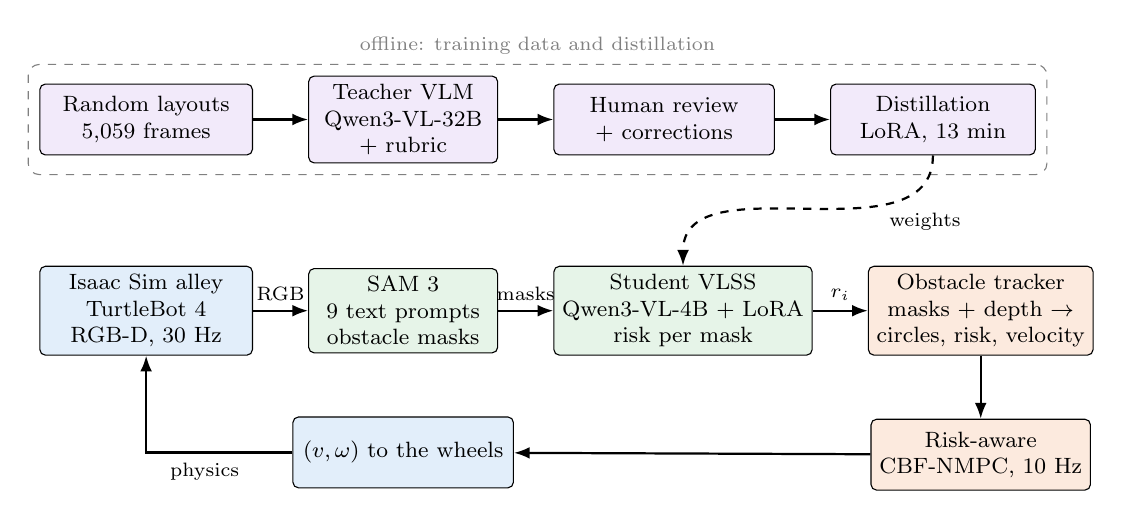
\begin{tikzpicture}[node distance=5mm and 7mm]
\node[box,fill=sim,minimum width=27mm] (sim) {Isaac Sim alley\\TurtleBot 4\\RGB-D, 30 Hz};
\node[box,fill=per,right=of sim,minimum width=24mm] (sam) {SAM 3\\9 text prompts\\obstacle masks};
\node[box,fill=per,right=of sam,minimum width=28mm] (vls) {Student VLSS\\Qwen3-VL-4B + LoRA\\risk per mask};
\node[box,fill=ctl,right=of vls,minimum width=26mm] (trk) {Obstacle tracker\\masks + depth $\to$\\circles, risk, velocity};
\node[box,fill=ctl,below=8mm of trk,minimum width=26mm] (mpc) {Risk-aware\\CBF-NMPC, 10 Hz};
\node[box,fill=sim,below=8mm of sam,minimum width=28mm] (cmd) {$(v,\omega)$ to the wheels};
\draw[arr] (sim) -- node[above,lab]{RGB} (sam);
\draw[arr] (sam) -- node[above,lab]{masks} (vls);
\draw[arr] (vls) -- node[above,lab]{$r_i$} (trk);
\draw[arr] (trk) -- (mpc);
\draw[arr] (mpc) -- (cmd);
\draw[arr] (cmd.west) -| node[pos=0.3,below,lab]{physics} (sim.south);
\node[box,fill=off,above=14mm of sim,minimum width=27mm] (lay) {Random layouts\\5{,}059 frames};
\node[box,fill=off,right=of lay,minimum width=24mm] (tea) {Teacher VLM\\Qwen3-VL-32B\\+ rubric};
\node[box,fill=off,right=of tea,minimum width=28mm] (rev) {Human review\\+ corrections};
\node[box,fill=off,right=of rev,minimum width=26mm] (trn) {Distillation\\LoRA, 13 min};
\draw[arr] (lay) -- (tea); \draw[arr] (tea) -- (rev); \draw[arr] (rev) -- (trn);
\draw[arr,dashed] (trn.south) to[out=-90,in=90] node[right,lab,pos=0.3,yshift=-2mm]{weights} (vls.north);
\begin{scope}[on background layer]
\node[draw=gray,dashed,rounded corners,fit=(lay)(tea)(rev)(trn),inner sep=4pt,label={[font=\scriptsize,gray]above:offline: training data and distillation}] {};
\end{scope}
\end{tikzpicture}
\caption{System overview. Offline (top), a large teacher model rates the obstacles in simulated frames, a human reviews the
ratings, and a small student model learns them. At runtime (bottom), SAM~3 segments, the student scores and the controller acts.}
\label{fig:overview}
\end{figure}

\paragraph{Terminology.} \emph{VLM}: vision-language model, image and text in, text out. \emph{VLA}: vision-language-action
model, a VLM whose output is a robot action instead of text, usually through a regression or action head. The student here is
built the same way as a VLA, but its head outputs a safety score per obstacle instead of an action; we call it a
vision-language \emph{safety scorer} model (VLSS).

\begin{center}\footnotesize
\begin{tabularx}{\textwidth}{>{\ttfamily}l X}
\toprule
\multicolumn{1}{l}{Folder} & Contents \\
\midrule
envs/ & Isaac Sim alley, the two scenarios, random layouts (\code{layout.py}), UR10e kinematics \\
perception/ & SAM~3 worker and client, ground test, student worker and client, drawing \\
distillation/ & teacher requests, label corrections, the student model with its data and metrics, progress files \\
control/ & CBF-NMPC (\code{cbf\_nmpc.py}) and the obstacle tracker (\code{obstacles.py}) \\
configs/ & environment (and the unseen scene), risk rubric and policy, student, controller \\
scripts/ & tests, dataset generation, labelling, training, evaluation, videos, tmux pipelines with progress bars \\
\bottomrule
\end{tabularx}\end{center}

%======================================================================================================================
\section{Simulation environment and data}

\subsection{Alley, robot and objects}
An 8~m $\times$ 2.2~m walled alley in Isaac Sim 5.1 / Isaac Lab 2.3; PhysX at 120~Hz, sensors and control at 30~Hz. The
TurtleBot~4 is imported from its URDF and driven through its wheel joints, so a command $(v,\omega)$ is subject to the Create~3
limits ($|v|\leq0.46$~m/s, $|\omega|\leq1.9$~rad/s, $|\dot v|\leq0.9$~m/s$^2$, $|\dot\omega|\leq4$~rad/s$^2$), wheel friction and
contacts. Footprint radius $\rho=0.172$~m. Camera: OAK-D Pro colour sensor, 640$\times$480, 69$^\circ$ horizontal field of view,
24~cm above the floor, with RGB and depth (distance to the image plane). Objects: two lidded buckets, a drinking glass on
Bucket~1, a glass vase, a leather sofa, an upholstered armchair, an ottoman on thin legs and a bean bag, all dynamic rigid bodies.

\paragraph{Scenarios.} \emph{person}: an animated person walks to Bucket~1, picks up the glass, carries it across the alley and
places it on the robot's side of Bucket~2 while the robot drives past. \emph{gripper\_robot}: a Jackal with a UR10e arm and a
Robotiq 2F-140 gripper does the same (inverse kinematics on the glass every physics step, 0.1~mm grasp error).

\subsection{Random layouts and frames}
\code{AlleyEnv.reset(layout)} rearranges the scene: which objects are present, where they stand, what stands on what (glass and
vase on a bucket, on a seat, on the floor, or held by the actor), bucket colours, glass tints, light intensity and sun
direction. Seat heights come from each furniture model's mesh (the 30th percentile of the surface height over the seat area);
objects are placed only where the cushion is flat. Per scenario the generator renders:
\begin{itemize}
\item 130 static layouts, each seen from 12 random robot viewpoints at 0.55--3.8~m from an object;
\item 48 \emph{extra} layouts (added for student v2) with the glass or vase on the sofa or armchair seat;
\item 6 episodes of the scripted transfer with the robot driving, one frame every 0.5~s.
\end{itemize}
A frame is kept if it shows an obstacle of at least 300 pixels. Each stores RGB, depth (uint16~mm), the simulator's instance
masks and the scene facts (pose, size, support relations).

\begin{center}\small
\begin{tabular}{lrrrrr}
\toprule
Split & train & val & test & test\_heldout & total \\
\midrule
frames & 4{,}031 & 336 & 452 & 240 & 5{,}059 \\
\bottomrule
\end{tabular}
\qquad 12{,}235 rated obstacles
\end{center}
Splits are assigned per \emph{layout}, so test frames never share a layout with training frames. \code{test\_heldout} contains an
arrangement that no other split has: the glass or the vase on the ottoman.

\subsection{Unseen scene}
\code{configs/env\_config\_ood.yaml} extends the base configuration with objects and materials the student never saw: two warehouse
pails (a blue plastic drum pail, a green pail with a handle) as buckets, a tufted Chesterfield sofa, a white upholstered armchair,
a leather ottoman on a swivel base, oak plank floor, stucco walls, granite caps and another sky. The orientation of new furniture
is found automatically: the side whose mesh is tallest becomes the backrest.

%======================================================================================================================
\section{Models: inputs, outputs and architecture}

\begin{center}\small
\begin{tabularx}{\textwidth}{l>{\raggedright}p{2.9cm}>{\raggedright}X>{\raggedright\arraybackslash}X}
\toprule
Model & Size & Input & Output \\
\midrule
SAM~3 (Meta) & 0.86~B params, 1.7~GB bf16 & RGB 640$\times$480 (resized to 1008$\times$1008) and 9 text prompts & per detected instance: binary mask 640$\times$480, box, score, prompt index \\
\addlinespace
Teacher VLM: Qwen3-VL-32B-Instruct (FP8) & 33~B params, 36~GB & system prompt (rubric); camera image 1280$\times$960; one $\approx$512~px close-up per obstacle; scene hints; JSON schema & JSON text: per obstacle name, what it carries, 4 booleans, reason, risk \\
\addlinespace
Student VLSS: Qwen3-VL-4B + LoRA + head & 4.48~B params (42~M trained), 9~GB bf16 & RGB 640$\times$480, fixed instruction, $K\le 8$ masks (as weights on the image tokens) and their geometry & per mask: risk $\in[0,1]$, 4 attribute probabilities \\
\addlinespace
CBF-NMPC & 25 steps, $\leq$16 obstacle circles & robot state, goal, obstacle circles with risk and velocity & velocity command $(v,\omega)$ \\
\bottomrule
\end{tabularx}
\end{center}

%----------------------------------------------------------------------------------------------------------------------
\subsection{SAM~3: promptable concept segmentation}

SAM~3 finds \emph{all} instances of a concept named by a short text prompt. Its image detector (used here; its video tracker is
not) is a DETR-style model conditioned on text:

\begin{figure}[H]
\centering
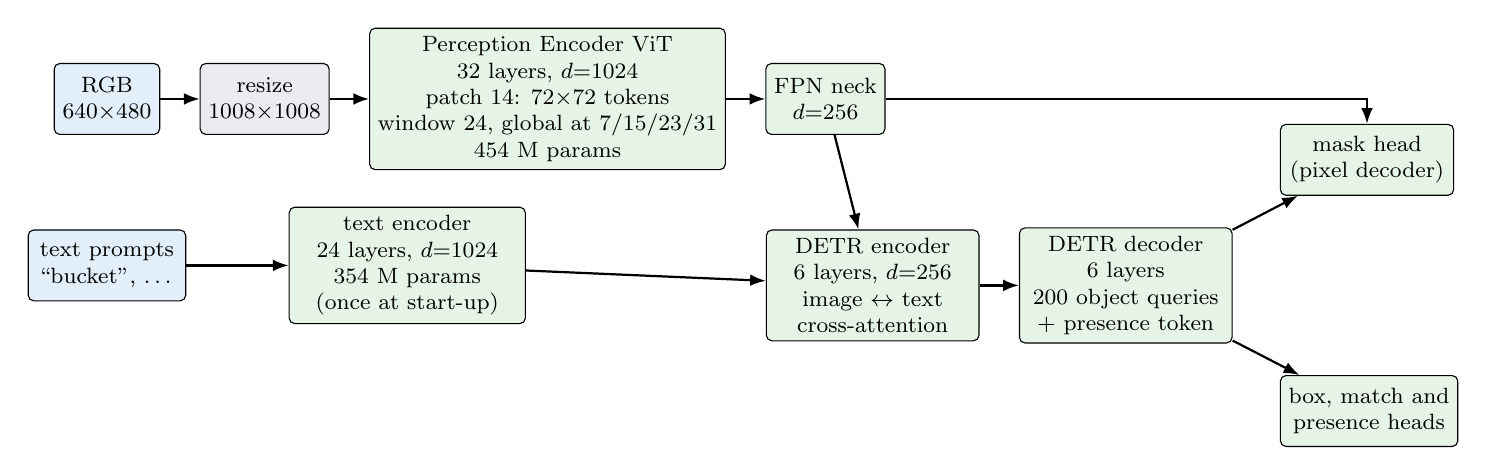
\begin{tikzpicture}[node distance=4mm and 5mm]
\node[box,fill=sim] (img) {RGB\\640$\times$480};
\node[box,fill=frz,right=of img] (rs) {resize\\1008$\times$1008};
\node[box,fill=per,right=of rs,minimum width=30mm] (vit) {Perception Encoder ViT\\32 layers, $d{=}1024$\\patch 14: $72{\times}72$ tokens\\window 24, global at 7/15/23/31\\454~M params};
\node[box,fill=per,right=of vit] (fpn) {FPN neck\\$d{=}256$};
\node[box,fill=sim,below=12mm of img,minimum width=20mm] (txt) {text prompts\\``bucket'', \dots};
\node[box,fill=per,right=of txt,minimum width=30mm,xshift=8mm] (te) {text encoder\\24 layers, $d{=}1024$\\354~M params\\(once at start-up)};
\node[box,fill=per,below=12mm of fpn,minimum width=27mm,xshift=6mm] (enc) {DETR encoder\\6 layers, $d{=}256$\\image $\leftrightarrow$ text\\cross-attention};
\node[box,fill=per,right=of enc,minimum width=27mm] (dec) {DETR decoder\\6 layers\\200 object queries\\+ presence token};
\node[box,fill=per,above right=4mm and 6mm of dec,minimum width=22mm] (mh) {mask head\\(pixel decoder)};
\node[box,fill=per,below right=4mm and 6mm of dec,minimum width=22mm] (bh) {box, match and\\presence heads};
\draw[arr] (img) -- (rs); \draw[arr] (rs) -- (vit); \draw[arr] (vit) -- (fpn); \draw[arr] (fpn) -- (enc);
\draw[arr] (txt) -- (te); \draw[arr] (te) -- (enc);
\draw[arr] (enc) -- (dec); \draw[arr] (dec) -- (bh); \draw[arr] (dec) -- (mh); \draw[arr] (fpn.east) -| (mh.north);
\end{tikzpicture}
\caption{SAM~3 image detector. Image features are computed once per frame and shared by all prompts; text features once at
start-up. Each object query predicts a box, a mask and a match logit; the presence token predicts whether the concept is in the
image at all.}
\end{figure}

\paragraph{Score.} For query $j$ and prompt $c$ the detection score separates recognition from localisation:
\begin{equation}
s_{j,c} = \sigma(\ell^{\text{presence}}_{c})\;\sigma(\ell^{\text{match}}_{j,c}).
\end{equation}

\paragraph{Our post-processing} (\code{perception/sam3\_worker.py}): keep $s\geq0.40$; mask probability $>0.5$ after resizing to
640$\times$480; masks of different prompts overlapping with IoU $\geq0.6$ are merged (higher score wins); at most 40 detections.
The nine prompts run as one batch over the shared image features. With \code{torch.compile} and CUDA graphs: 49~ms per frame on an
RTX PRO 6000 (20 FPS).

\paragraph{Obstacle test.} A detection is an obstacle when a visible part of it is low enough to hit. Each mask pixel $(u,v)$
with depth $z$ is back-projected with the intrinsics $K$ and the camera pose $T_{wc}=(R,t)$:
\begin{equation}
\bm p_c = z\,K^{-1}\begin{bmatrix}u\\v\\1\end{bmatrix},\qquad \bm p_w = R\,\bm p_c + t,\qquad
\text{obstacle} \iff \operatorname{perc}_{2}\{p_{w,z}\} < 0.35~\text{m}.
\end{equation}
The 2nd percentile ignores a few pixels spilling onto the floor; 0.35~m is the robot's height. It keeps the glass on a bucket or
in a hand out and keeps a sofa in when its legs are hidden. Against the exact masks SAM~3 finds 93\,\% of the obstacles in the
test frames (IoU $\geq0.5$) and 84\,\% in the unseen scene.

%----------------------------------------------------------------------------------------------------------------------
\subsection{Teacher VLM: Qwen3-VL-32B}

The teacher runs only offline, on the lab's vLLM server (OpenAI-compatible API, FP8 weights, 4 requests in parallel, 1.45~s
per frame). It applies a written rubric (Appendix~\ref{app:rubric}) to each frame.

\begin{figure}[H]
\centering
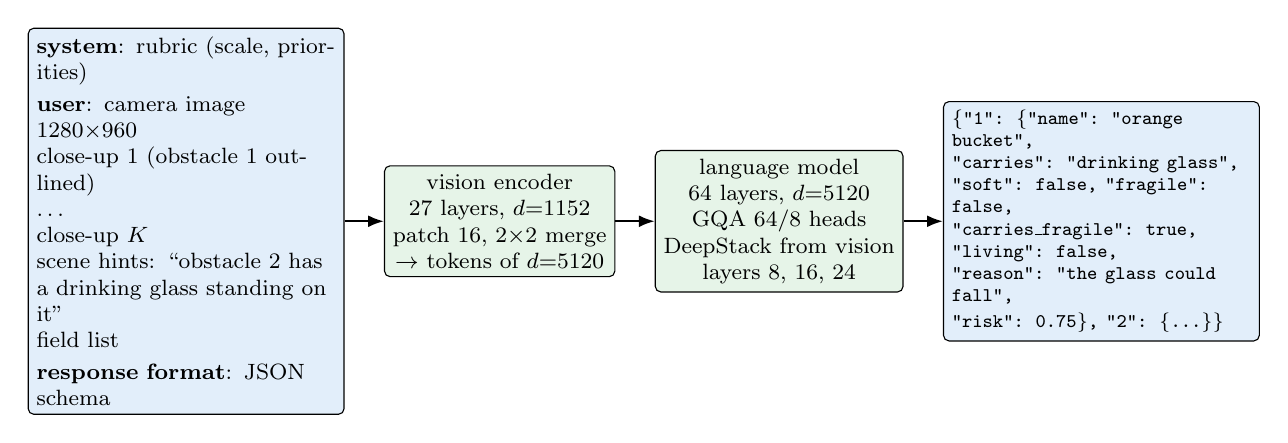
\begin{tikzpicture}[node distance=3mm and 5mm]
\node[box,fill=sim,text width=38mm,align=left] (in) {\textbf{system}: rubric (scale, priorities)\\[2pt]
\textbf{user}: camera image 1280$\times$960\\
close-up 1 (obstacle 1 outlined)\\
\dots\\ close-up $K$\\
scene hints: ``obstacle 2 has a drinking glass standing on it''\\
field list\\[2pt]
\textbf{response format}: JSON schema};
\node[box,fill=per,right=of in,minimum width=28mm] (vit) {vision encoder\\27 layers, $d{=}1152$\\patch 16, $2{\times}2$ merge\\$\to$ tokens of $d{=}5120$};
\node[box,fill=per,right=of vit,minimum width=28mm] (lm) {language model\\64 layers, $d{=}5120$\\GQA 64/8 heads\\DeepStack from vision\\layers 8, 16, 24};
\node[box,fill=sim,right=of lm,text width=38mm,align=left] (out) {\ttfamily\scriptsize\{"1": \{"name": "orange bucket",\\
"carries": "drinking glass",\\ "soft": false, "fragile": false,\\ "carries\_fragile": true,\\ "living": false,\\ "reason": "the glass could fall",\\ "risk": 0.75\}, "2": \{\dots\}\}};
\draw[arr] (in) -- (vit); \draw[arr] (vit) -- (lm); \draw[arr] (lm) -- (out);
\end{tikzpicture}
\caption{One teacher request. Close-ups are cut from the camera image around each obstacle (a square reaching one obstacle height
above it), enlarged to about 512~px, with that obstacle alone outlined from the simulator's exact mask. Decoding is greedy
(temperature 0) and the JSON schema is enforced by vLLM, so the reason is written before the number.}
\end{figure}

\paragraph{Which obstacles are rated.} Objects with $\geq$300 visible pixels whose base is below 0.35~m and of which at least
25\,\% is visible (estimated as the pixel count over the area of the object's silhouette at that distance,
$\approx f^2 A/d^2$), unless they cover $\geq$4{,}000 pixels.

\paragraph{Scene hints.} A pilot on 64 frames: with the image and close-ups alone, the teacher noticed the glass on a bucket in
27\,\% of frames (with 1920$\times$1440 renders: 55\,\%); told what the simulator knows stands on each obstacle, 100\,\%, and every
bucket with a glass was rated inside 0.60--0.85. The hints are privileged information for the teacher only; they name things,
never risks, and the student never sees them.

\paragraph{Review and corrections.} 64 frames covering every obstacle state were reviewed on a web page; the reviewer raised the
gripper robot and the glass on the floor. The corrected label $\tilde r$ follows from the teacher's $r$, the policy range $[l_s,h_s]$
of the obstacle's state $s$, and whether the teacher's description names the object:
\begin{equation}
\tilde r = \begin{cases}
r_{\text{reviewer}} & \text{if the reviewer set it}\\
r & \text{if } r\in[l_s,h_s]\\
\min(\max(r,l_s),h_s) & \text{if the teacher recognised the object}\\
\operatorname{median}\{r' : \text{in-range ratings of state } s\} & \text{otherwise (it rated a neighbour)}
\end{cases}
\end{equation}
Of 12{,}235 ratings: 9{,}943 kept, 2{,}023 clipped, 258 replaced, 11 reviewer values.

\begin{center}\small
\begin{tabular}{lcl}
\toprule
Obstacle state $s$ & $[l_s,h_s]$ & Reason \\
\midrule
sofa, armchair, ottoman, bean bag & 0.00--0.15 & soft, yields \\
bucket (nothing on it) & 0.15--0.35 & rigid, may be pushed \\
gripper robot & 0.65--0.75 & hard and heavy: damages the TurtleBot \\
anything carrying a glass or vase & 0.60--0.85 & the glass can fall \\
glass or vase on the floor & 0.80--0.90 & hit directly: breaks \\
gripper robot holding the glass & 0.80--0.90 & both of the above \\
person, with or without the glass & 0.90--1.00 & a living being \\
\bottomrule
\end{tabular}
\end{center}

%----------------------------------------------------------------------------------------------------------------------
\subsection{Student VLS: Qwen3-VL-4B with query tokens and a score head}\label{sec:student}

\begin{figure}[H]
\centering
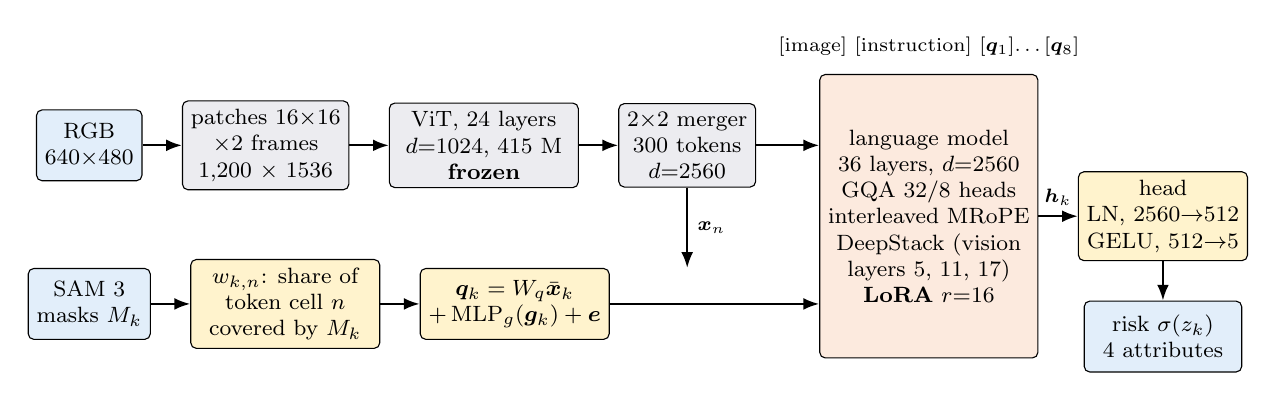
\begin{tikzpicture}[node distance=4mm and 5mm]
\node[box,fill=sim] (img) {RGB\\640$\times$480};
\node[box,fill=frz,right=of img] (pe) {patches $16{\times}16$\\$\times$2 frames\\1{,}200 $\times$ 1536};
\node[box,fill=frz,right=of pe,minimum width=24mm] (vit) {ViT, 24 layers\\$d{=}1024$, 415~M\\\textbf{frozen}};
\node[box,fill=frz,right=of vit] (mg) {$2{\times}2$ merger\\300 tokens\\$d{=}2560$};
\node[box,fill=sim,below=11mm of img] (msk) {SAM 3\\masks $M_k$};
\node[box,fill=trn,right=of msk,minimum width=24mm] (pool) {$w_{k,n}$: share of\\token cell $n$\\covered by $M_k$};
\node[box,fill=trn,right=of pool,minimum width=24mm] (q) {$\bm q_k = W_q\bar{\bm x}_k$\\$+\,\mathrm{MLP}_g(\bm g_k) + \bm e$};
\node[box,fill=ctl,right=8mm of mg,minimum height=36mm,minimum width=27mm,yshift=-9mm] (lm) {language model\\36 layers, $d{=}2560$\\GQA 32/8 heads\\interleaved MRoPE\\DeepStack (vision\\layers 5, 11, 17)\\\textbf{LoRA} $r{=}16$};
\node[box,fill=trn,right=of lm,minimum width=20mm] (hd) {head\\LN, 2560$\to$512\\GELU, 512$\to$5};
\node[box,fill=sim,below=5mm of hd,minimum width=20mm] (o) {risk $\sigma(z_k)$\\4 attributes};
\draw[arr] (img) -- (pe); \draw[arr] (pe) -- (vit); \draw[arr] (vit) -- (mg);
\draw[arr] (msk) -- (pool); \draw[arr] (pool) -- (q); \draw[arr] (mg.south) -- node[right,lab]{$\bm x_n$} (q.north -| mg.south);
\draw[arr] (mg.east) -- (lm.west |- mg.east); \draw[arr] (q.east) -- (lm.west |- q.east);
\draw[arr] (lm) -- node[above,lab]{$\bm h_k$} (hd); \draw[arr] (hd) -- (o);
\node[lab,above=1mm of lm] {[image] [instruction] [$\bm q_1$]\dots[$\bm q_8$]};
\end{tikzpicture}
\caption{The student. Grey: frozen; yellow: trained from scratch; orange: frozen weights with trained LoRA adapters. One forward
pass, no text generation.}
\end{figure}

\paragraph{Image tokens.} The 640$\times$480 image is cut into $16{\times}16$ patches (duplicated in time, as Qwen3-VL treats an
image as a two-frame video): 1{,}200 vectors of $3\cdot2\cdot16\cdot16=1536$ values, projected to $d=1024$, encoded by 24
transformer layers and merged in $2{\times}2$ groups into $N=15\times20=300$ tokens $\bm x_n\in\R^{2560}$, each covering a
$32{\times}32$-pixel cell.

\paragraph{Query tokens.} For mask $M_k$, the share of each token cell $C_n$ it covers, its mean image feature and its geometry:
\begin{equation}
w_{k,n} = \frac{|M_k\cap C_n|}{|C_n|},\qquad
\bar{\bm x}_k = \frac{\sum_n w_{k,n}\,\bm x_n}{\sum_n w_{k,n}},\qquad
\bm g_k = \big(u_0,v_0,u_1,v_1,\sqrt{a},\bar u,\bar v,v_{98}\big)\in[0,1]^8
\end{equation}
(box, square root of the area fraction, centroid, 98th-percentile row, all normalised by the image size), and
\begin{equation}
\bm q_k = W_q\,\bar{\bm x}_k + \mathrm{MLP}_g(\bm g_k) + \bm e,
\end{equation}
with $W_q$ initialised to the identity, the last layer of $\mathrm{MLP}_g$ to zero and $\bm e$ to the embedding of an unused
token, so that at the start $\bm q_k$ is the object's own mean feature.

\paragraph{Sequence and attention.} The language model reads [image tokens][instruction][$\bm q_1,\dots,\bm q_8$] with causal
attention:
\begin{equation}
\mathrm{Attn}(Q,K,V) = \mathrm{softmax}\!\Big(\frac{QK^\top}{\sqrt{d_h}} + C\Big)V,\qquad C_{ij} = \begin{cases}0 & j\leq i\\ -\infty & j>i\end{cases}
\end{equation}
Each query therefore attends to the whole image, to the instruction and to the earlier queries: the score of a bucket can use the
pixels of the glass standing on it, which are outside the bucket's mask. Unused query slots come last and cannot influence used
ones. Qwen3-VL's DeepStack adds features from vision layers 5, 11 and 17 to the image positions of the first three language
layers; positions use interleaved multimodal rotary embeddings (time, row, column).

\paragraph{Head.} From the last hidden state $\bm h_k$ of query $k$:
\begin{equation}
[z_k, \bm a_k] = W_2\,\mathrm{GELU}\big(W_1\,\mathrm{LN}(\bm h_k)\big),\qquad \hat r_k = \sigma(z_k),\qquad
\hat{\bm\alpha}_k = \sigma(\bm a_k)\in[0,1]^4
\end{equation}
for the risk and the attributes \emph{soft, fragile, carries fragile, living}.

\paragraph{LoRA.} Every attention projection ($q,k,v,o$) and MLP projection (gate, up, down) of the 36 language layers gets
$W' = W + \tfrac{\alpha}{r}BA$ with $A\in\R^{r\times d_{in}}$, $B\in\R^{d_{out}\times r}$, $r=16$, $\alpha=32$, dropout 0.05;
$W$ stays frozen. Trainable: 41.6~M parameters (LoRA, $W_q$, $\mathrm{MLP}_g$, $\bm e$, head) of 4.48~B. For inference the
adapters are merged into $W$.

\paragraph{A speed fix.} Qwen3-VL's patch embedding is a \code{Conv3d} whose kernel equals its stride. In bfloat16 cuDNN has no
fast path for it on this GPU: 5~s per image. It is replaced by the identical matrix product $\bm y = W\,\mathrm{vec}(\text{patch})+b$
(difference $3\cdot10^{-6}$), which takes well under 1~ms.

%======================================================================================================================
\section{Training methodology}

\paragraph{Samples.} One sample is one frame with up to 8 of its rated obstacles. For each obstacle the mask is SAM~3's own mask
(precomputed for all frames, matched to the object at IoU $\geq0.5$) with probability 0.8 when SAM~3 found it, otherwise the
simulator's exact mask; the student thus learns on the masks it will get at runtime, including their errors. Augmentation:
horizontal flip of image and masks ($p=0.5$), per-channel gain and offset ($\pm15\,\%$).

\paragraph{Loss.} With targets $\tilde r_k$ (corrected labels), the teacher's attributes $\bm\alpha_k$ and the valid queries
$\mathcal V$ of a batch:
\begin{align}
\mathcal L_{\text{risk}} &= \frac{1}{|\mathcal V|}\sum_{k\in\mathcal V}\frac{1}{\delta}\,\mathrm{Huber}_\delta(\hat r_k-\tilde r_k),\qquad
\mathrm{Huber}_\delta(e)=\begin{cases}\tfrac12 e^2 & |e|\leq\delta\\ \delta(|e|-\tfrac12\delta) & \text{else}\end{cases},\quad \delta=0.1\\
\mathcal L_{\text{rank}} &= \frac{1}{|\mathcal P|}\sum_{(i,j)\in\mathcal P}\log\big(1+e^{-(z_i-z_j)}\big),\qquad
\mathcal P=\{(i,j)\ \text{in the same frame}: \tilde r_i-\tilde r_j\geq0.10\}\\
\mathcal L_{\text{attr}} &= \frac{1}{4|\mathcal V|}\sum_{k\in\mathcal V}\sum_{m=1}^{4}\mathrm{BCE}(\hat\alpha_{k,m},\alpha_{k,m})\\
\mathcal L &= 1.0\,\mathcal L_{\text{risk}} + 0.5\,\mathcal L_{\text{rank}} + 0.2\,\mathcal L_{\text{attr}}.
\end{align}
The Huber term fits the values, the ranking term the order within a frame (which is what the controller acts on), and the
attribute term gives the representation a reason for its score.

\paragraph{Optimisation.} AdamW ($\beta=(0.9,0.999)$, weight decay 0.01), gradient norm clipped to 1, batch 8, bfloat16 autocast
with fp32 trainable weights, 4 epochs (v2: 2{,}012 steps, 13~minutes on one RTX PRO 6000 Blackwell with 96~GB). Learning rate
\begin{equation}
\eta(s) = \eta_0\,\min\!\Big(1,\frac{s+1}{100}\Big)\,\tfrac12\Big(1+\cos\frac{\pi s}{S}\Big),\qquad \eta_0=2\cdot10^{-4}.
\end{equation}
The checkpoint with the lowest validation MAE (SAM~3 masks), evaluated every 200 steps, is kept.

\paragraph{Two versions.} v1 trained on 3{,}908 frames in which only buckets carry anything. v2 added the 1{,}151 extra frames
(glass or vase on the sofa and armchair seats), labelled with rubric v2.

%======================================================================================================================
\section{Testing methodology}

\begin{itemize}
\item \textbf{Splits by layout.} val (model selection), test (unseen layouts), test\_heldout (glass or vase on the ottoman, never in
training), and the \textbf{unseen scene} (new objects and materials; 1{,}152 frames from 96 layouts).
\item \textbf{Masks.} Each test runs twice: with SAM~3's masks (what the robot sees; obstacles SAM~3 missed are counted
separately) and with the exact masks (the model alone).
\item \textbf{Against labels:} $\mathrm{MAE}=\frac1n\sum|\hat r-\tilde r|$; the share within 0.10; pair accuracy
$=\frac{|\{(i,j)\in\mathcal P:\hat r_i>\hat r_j\}|}{|\mathcal P|}$.
\item \textbf{Against the policy} (no labels needed, so it works in the unseen scene): a score is inside when
$\hat r\in[l_s-0.05,\,h_s+0.05]$; the distance outside is $\max(l_s-0.05-\hat r,\ \hat r-h_s-0.05,\ 0)$.
\item \textbf{Gate} for using the student: test MAE $\leq0.08$, pair accuracy $\geq90\,\%$, latency $\leq50$~ms.
\item \textbf{Videos:} driving runs in both scenarios, with per-frame scores coloured on the masks and checked against the policy range.
\item \textbf{Closed loop:} the CBF-NMPC with simulator obstacles and policy risks, with a uniform risk of 0.5 (no semantics), and
with the full pipeline; metrics are the minimum gap to every object, contacts, the glass's final support, time to the goal and
solver statistics.
\end{itemize}

%======================================================================================================================
\section{Results}

\subsection{Student against the corrected labels}
\begin{center}\small
\begin{tabular}{lrcccccc}
\toprule
 & & \multicolumn{3}{c}{v1 (only buckets carry things)} & \multicolumn{3}{c}{v2 (+ glass/vase on seats)} \\
\cmidrule(lr){3-5}\cmidrule(lr){6-8}
Split, SAM 3 masks & obstacles & MAE & within 0.10 & pairs & MAE & within 0.10 & pairs \\
\midrule
val & 744 & 0.070 & 84.5\,\% & 96.1\,\% & 0.057 & 86.0\,\% & 98.4\,\% \\
test & 1{,}051 & 0.066 & 83.2\,\% & 97.1\,\% & \textbf{0.052} & 85.3\,\% & \textbf{99.6\,\%} \\
test\_heldout & 480 & 0.137 & 79.2\,\% & 80.6\,\% & \textbf{0.077} & 85.0\,\% & \textbf{89.3\,\%} \\
\bottomrule
\end{tabular}
\end{center}
With exact masks the numbers are within 0.001 MAE: SAM~3's masks cost the student almost nothing. v2 passes the gate on test, and
the MAE part on test\_heldout (its pair accuracy, 89.3\,\%, is just under 90\,\%).

\subsection{Against the policy: per obstacle, normal test frames and the unseen scene}
\begin{center}\small
\begin{tabular}{lcrccrcc}
\toprule
 & & \multicolumn{3}{c}{test + test\_heldout} & \multicolumn{3}{c}{unseen scene} \\
\cmidrule(lr){3-5}\cmidrule(lr){6-8}
Obstacle state & range & $n$ & v1 & v2 & $n$ & v1 & v2 \\
\midrule
armchair & 0.00--0.15 & 143 & 0.12 & 0.15 & 302 & 0.15 & 0.19 \\
couch & 0.00--0.15 & 195 & 0.10 & 0.12 & 313 & 0.12 & 0.14 \\
ottoman & 0.00--0.15 & 79 & 0.06 & 0.06 & 62 & 0.21 & 0.18 \\
bean bag & 0.00--0.15 & 142 & 0.05 & 0.05 & 193 & 0.04 & 0.05 \\
bucket & 0.15--0.35 & 374 & 0.24 & 0.23 & 483 & 0.23 & 0.22 \\
gripper robot & 0.65--0.75 & 102 & 0.67 & 0.67 & 167 & 0.68 & 0.68 \\
bucket + drinking glass & 0.60--0.85 & 93 & 0.80 & 0.80 & 197 & 0.70 & 0.69 \\
bucket + glass vase & 0.60--0.85 & 16 & 0.70 & 0.78 & 83 & 0.76 & 0.73 \\
armchair or couch + glass or vase & 0.60--0.85 & 32 & 0.12 & 0.70 & -- & -- & -- \\
ottoman + glass or vase (held out) & 0.60--0.85 & 71 & 0.08 & 0.51 & 7 & 0.22 & 0.76 \\
glass vase on the floor & 0.80--0.90 & 84 & 0.88 & 0.87 & 192 & 0.89 & 0.88 \\
drinking glass on the floor & 0.80--0.90 & 13 & 0.85 & 0.86 & 40 & 0.87 & 0.87 \\
gripper robot + glass & 0.80--0.90 & 28 & 0.79 & 0.80 & 27 & 0.79 & 0.80 \\
person (with or without the glass) & 0.90--1.00 & 159 & 1.00 & 1.00 & 207 & 1.00 & 1.00 \\
\midrule
\multicolumn{2}{l}{share of scores inside the range} & 1{,}531 & 89.2\,\% & \textbf{92.4\,\%} & 2{,}273 & 93.7\,\% & \textbf{91.9\,\%} \\
\bottomrule
\end{tabular}
\end{center}
Columns v1 and v2 are mean scores. In the unseen scene both students keep their behaviour on new buckets, sofas and floors
(92--94\,\% inside); v2's small drop there is the new white armchair, rated 0.19 (slightly cautious). The test that matters,
something fragile on a support never seen in training, is passed only by v2, and only partly: the ottoman with a glass or vase
gets 0.51 on test\_heldout (v1: 0.08; 59\,\% inside the range) and 0.76 in the unseen scene (v1: 0.22; only 7 cases there).

\subsection{Driving videos}
\begin{center}\small
\begin{tabular}{llcc}
\toprule
Video & Obstacle & v1 mean (inside) & v2 mean (inside) \\
\midrule
person, default scene & bucket + glass & 0.81 (93\,\%) & 0.79 (93\,\%) \\
 & person & 1.00 (99\,\%) & 1.00 (99\,\%) \\
 & sofa / ottoman / bucket & 0.14 / 0.08 / 0.22 & 0.16 / 0.01 / 0.21 \\
person, vase on the ottoman (held out) & ottoman + vase & \textbf{0.04 (0\,\%)} & \textbf{0.82 (94\,\%)} \\
gripper robot, default scene & gripper robot / + glass & 0.66 / 0.81 & 0.67 / 0.82 \\
\bottomrule
\end{tabular}
\end{center}
Recordings: \code{recordings/risk\_student\_v\{1,2\}\_*.mp4}. The videos in the unseen scene have not been recorded yet (the first
attempt ran out of GPU memory next to the controller runs).

%======================================================================================================================
\section{Runtime, model size and embedded deployment}\label{sec:runtime}

\subsection{Measured on the workstation}
\begin{center}\small
\begin{tabular}{lrrl}
\toprule
Stage (RTX PRO 6000 Blackwell, one process) & median & rate & note \\
\midrule
SAM~3, 9 prompts, compiled & 49~ms & 20~Hz & 70--99~ms with 3 runs sharing the GPU \\
Student v2, 6 obstacles, incl.\ preprocessing & 29~ms & 34~Hz & p95 30~ms \\
Perception total (SAM~3, then student) & 78~ms & 13~Hz & \\
CBF-NMPC solve (IPOPT, one CPU core) & 24--28~ms & 10~Hz used & p95 37~ms (person runs) \\
Teacher (offline) & 1.45~s & & 4 requests in parallel \\
\bottomrule
\end{tabular}
\end{center}

\subsection{Can it run on a Jetson in real time?}
Not measured; estimated from the compute per frame. Student: vision $2\times0.415\,\text{B}\times1200\approx1.0$~TFLOP, language
model $2\times3.6\,\text{B}\times340$ tokens $\approx2.5$~TFLOP, about 3.5~TFLOP per frame (the workstation sustains about
120~TFLOP/s on it). SAM~3: $2\times0.454\,\text{B}\times5184$ tokens $\approx4.7$~TFLOP per frame. Assuming 40\,\% of the dense
FP16/BF16 tensor throughput is reached:

\begin{center}\small
\begin{tabular}{lcccccc}
\toprule
Device & memory & dense FP16 & student 4B & SAM~3 & both & student 0.8B \\
\midrule
RTX PRO 6000 (measured) & 96~GB & -- & 29~ms & 49~ms & 13~Hz & 22~ms \\
Jetson AGX Thor & 128~GB & $\sim$250~TFLOPS & $\sim$35~ms & $\sim$50~ms & $\sim$10~Hz & $\sim$10~ms \\
Jetson AGX Orin 64~GB & 64~GB & $\sim$40~TFLOPS & $\sim$200~ms & $\sim$300~ms & $\sim$2~Hz & $\sim$40~ms \\
Jetson Orin NX 16~GB & 16~GB & $\sim$15~TFLOPS & $\sim$0.6~s & $\sim$0.8~s & $<$1~Hz & $\sim$110~ms \\
Jetson Orin Nano 8~GB & 8~GB & $\sim$8~TFLOPS & does not fit in bf16 & $\sim$1.5~s & -- & $\sim$0.2~s \\
\bottomrule
\end{tabular}
\end{center}
\textbf{So:} the present 4B student with SAM~3 is real-time only on a Jetson AGX Thor class device. On an AGX Orin it would run
at about 2~Hz, which is usable if the tracker carries the scores between updates (risk changes slowly; geometry comes from depth at
30~Hz) but not for fast dynamic scenes. To reach 10~Hz on Orin: (1) the 0.8B student (Qwen3.5-0.8B, about 0.65~TFLOP per frame);
(2) TensorRT with INT8/FP8 weights (about 2$\times$); (3) a lighter segmenter than SAM~3, SAM~3 at a lower resolution, or SAM~3 at
a few Hz with mask propagation in between; (4) scoring only new or changed tracks. Memory: the 4B student needs 9~GB in bf16,
2.5~GB in 4-bit. The controller (IPOPT, 25~ms on the workstation CPU) would take roughly 3$\times$ longer on Orin's Arm cores;
a real-time-iteration solver such as acados needs about 1--3~ms.

%======================================================================================================================
\section{Risk-aware CBF-NMPC}

\begin{figure}[H]
\centering
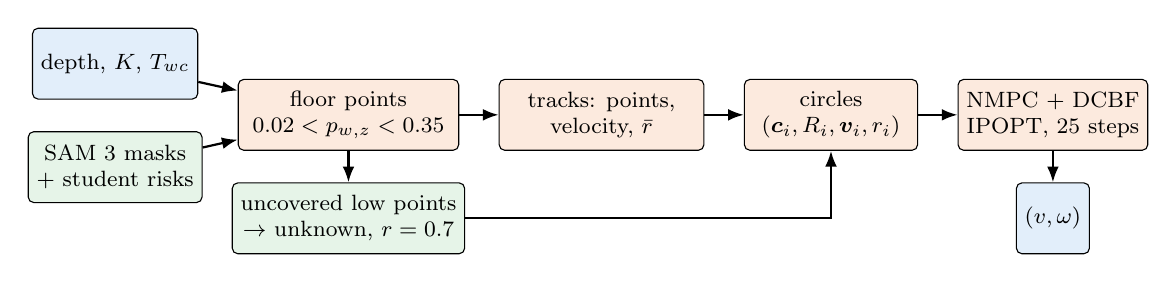
\begin{tikzpicture}[node distance=4mm and 5mm]
\node[box,fill=sim] (dep) {depth, $K$, $T_{wc}$};
\node[box,fill=per,below=of dep] (ms) {SAM 3 masks\\+ student risks};
\node[box,fill=ctl,right=of dep,yshift=-6.5mm,minimum width=28mm] (fp) {floor points\\$0.02<p_{w,z}<0.35$};
\node[box,fill=ctl,right=of fp,minimum width=26mm] (tr) {tracks: points,\\velocity, $\bar r$};
\node[box,fill=ctl,right=of tr,minimum width=22mm] (ci) {circles\\$(\bm c_i,R_i,\bm v_i,r_i)$};
\node[box,fill=ctl,right=of ci,minimum width=24mm] (np) {NMPC + DCBF\\IPOPT, 25 steps};
\node[box,fill=sim,below=of np] (u) {$(v,\omega)$};
\node[box,fill=per,below=of fp,minimum width=28mm] (un) {uncovered low points\\$\to$ unknown, $r=0.7$};
\draw[arr] (dep) -- (fp); \draw[arr] (ms) -- (fp); \draw[arr] (fp) -- (tr); \draw[arr] (tr) -- (ci); \draw[arr] (ci) -- (np); \draw[arr] (np) -- (u);
\draw[arr] (fp) -- (un); \draw[arr] (un.east) -| (ci.south);
\end{tikzpicture}
\caption{From perception to commands. With simulator obstacles (to test the controller alone) the circles come directly from the
objects' poses and sizes.}
\end{figure}

\subsection{Model and cost}
State $\bm x=[p_x,p_y,\theta,v,\omega]^\top$, input $\bm u=[a,\alpha]^\top$; the velocities are states so that the acceleration
limits hold:
\begin{equation}
\dot{\bm x} = f(\bm x,\bm u) = [\,v\cos\theta,\ v\sin\theta,\ \omega,\ a,\ \alpha\,]^\top,
\end{equation}
discretised with fourth-order Runge--Kutta, $\Delta t=0.12$~s, $N=25$ (3~s ahead), re-solved every 0.1~s from the measured state
and warm-started from the previous solution shifted by one step. With goal $\bm g$:
\begin{equation}
J=\sum_{k=0}^{N-1}\Big(\|\bm p_{k+1}-\bm g\|^2 + 0.3\,p_{y,k+1}^2 + 0.5\,a_k^2 + 0.05\,\alpha_k^2 + 0.2\,\omega_{k+1}^2\Big)
+ 20\,\|\bm p_N-\bm g\|^2 + \sum_{i,k}\big(200\,s_{i,k}^2 + 20\,s_{i,k}\big).
\end{equation}
Bounds: $-0.05\leq v_k\leq0.30$~m/s (capped below the robot's 0.46 so the scripted actors still meet it), $|\omega_k|\leq1.9$,
$|a_k|\leq0.9$, $|\alpha_k|\leq4$, all for $k\geq1$ (the measured initial state can exceed a bound slightly, and bounding it made
40\,\% of the problems infeasible); walls: $|p_{y,k}|\leq1.1-\rho-0.03$.

\subsection{Barrier functions with risk}
Obstacle $i$ is a circle with centre $\bm c_i$, radius $R_i$, velocity $\bm v_i$ (constant over the horizon) and risk $r_i$:
\begin{equation}
d_{i,k} = \big\|\bm p_k - (\bm c_i + k\,\Delta t\,\bm v_i)\big\|,\qquad
h_{i,k} = d_{i,k} - \big(\rho + R_i + m(r_i)\big).
\end{equation}
\textbf{Contact constraint (hard):} $d_{i,k+1}\geq\rho+R_i+m_0$ with $m_0=0.01$~m, whatever the risk.\\
\textbf{Risk barrier (soft):} the discrete-time CBF condition with slack $s_{i,k}\geq0$,
\begin{equation}
h_{i,k+1}\geq(1-\gamma(r_i))\,h_{i,k} - s_{i,k},\qquad 0<\gamma\leq1.
\end{equation}
Without slack it gives $h_{i,k}\geq(1-\gamma)^k h_{i,0}$: if the robot starts outside the risk margin ($h_{i,0}\geq0$) it stays
outside (forward invariance), and if it starts inside, the violation may grow by at most the factor $(1-\gamma)$ per step relative
to its current value, so the robot cannot dive deeper in quickly. The risk sets both how far and how fast:
\begin{equation}
m(r) = 0.03 + 0.32\,r~\text{m},\qquad \gamma(r) = 0.70 - 0.55\,r .
\end{equation}
A sofa ($r\approx0.07$) may be passed 5~cm away and approached quickly ($\gamma=0.66$); a person ($r\approx0.95$) is kept 33~cm
away and approached slowly ($\gamma=0.18$). The slack lets the risk margin give way where the alley is too narrow for it (between
the vase and Bucket~1 only 0.14~m remain beyond the robot's width), in proportion to its penalty; the contact constraint never
gives way. $h$ is in metres rather than squared metres: with $d^2$ a centimetre of intrusion cost more for a large obstacle, and
the robot gave a small high-risk vase less room than a large low-risk bucket.

\begin{figure}[H]
\centering
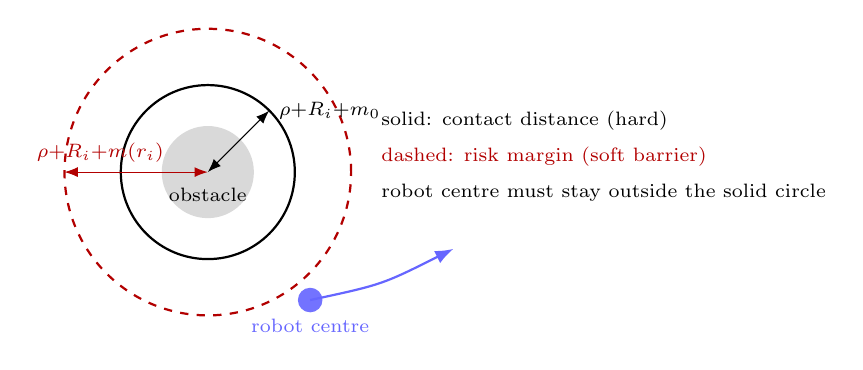
\begin{tikzpicture}[scale=1.3]
\fill[gray!30] (0,0) circle (0.45); \node[font=\scriptsize] at (0,-0.22) {obstacle};
\draw[thick] (0,0) circle (0.85);
\draw[dashed,thick,red!70!black] (0,0) circle (1.4);
\draw[{Latex}-{Latex}] (0,0) -- (0.6,0.6) node[pos=1,right,font=\scriptsize]{$\rho{+}R_i{+}m_0$};
\draw[{Latex}-{Latex},red!70!black] (0,0) -- (-1.4,0) node[pos=0.75,above,font=\scriptsize]{$\rho{+}R_i{+}m(r_i)$};
\node[font=\scriptsize,align=left,anchor=west] at (1.6,0.5) {solid: contact distance (hard)};
\node[font=\scriptsize,align=left,anchor=west,red!70!black] at (1.6,0.15) {dashed: risk margin (soft barrier)};
\node[font=\scriptsize,align=left,anchor=west] at (1.6,-0.2) {robot centre must stay outside the solid circle};
\fill[blue!55] (1.0,-1.25) circle (0.12);
\draw[-{Latex},blue!60,thick] (1.0,-1.25) .. controls (1.7,-1.1) .. (2.4,-0.75);
\node[font=\scriptsize,blue!60] at (1.0,-1.5) {robot centre};
\end{tikzpicture}
\caption{The two constraints around one obstacle (the robot's radius $\rho$ is added to the obstacle's).}
\end{figure}

\subsection{Obstacle tracker (full pipeline)}
Every obstacle mask's depth pixels between 2~cm and 0.35~m above the floor (within 4~m) are projected to the floor (Section~3.1)
and down-sampled on a 4~cm grid. A detection joins the track with a floor point within 0.35~m; a still track accumulates points
(it stays known after leaving the 69$^\circ$ view), a moving one keeps only the latest. Velocity:
$\bm v\leftarrow0.7\bm v+0.3\,\Delta\bm c/\Delta t$ when the centre moves more than 3~cm per update; risk:
$\bar r\leftarrow0.7\bar r+0.3\,\hat r$. A track's points are split along their main axis into pieces of at most 0.3~m, each
covered by a circle around its points plus 5~cm (the unseen back). Low points that no mask covers, away from the walls, are
clustered into unknown obstacles with risk 0.7. Simulator furniture is covered by circles at most 0.25~m apart along its long
side, so that they bulge at most a few centimetres into the aisle.

\subsection{Closed-loop results}\label{sec:closed}
Kinematic test (ideal unicycle, simulator obstacle layout, policy risks against one risk of 0.5):
\begin{center}\small
\begin{tabular}{llll}
\toprule
Glass on & risk & passes the sofa / Bucket~2 at $p_y$ & closest gaps \\
\midrule
Bucket~2 & semantic & $+0.06$ (beside the sofa) & sofa 0.05, Bucket~2 0.16 \\
Bucket~2 & uniform & $-0.04$ (middle) & Bucket~2 0.01 \\
Bucket~1 & semantic & splits the gap B1 / vase: 0.08 / 0.06 & \\
\bottomrule
\end{tabular}
\end{center}

In Isaac Sim (TurtleBot dynamics, scripted actor moving the glass):
\begin{center}\small
\begin{tabular}{llcccccc}
\toprule
Scenario & risk & goal & Bucket~2 (glass) & sofa & person / robot & vase & converged \\
\midrule
person & uniform 0.5 & 23.6~s & 0.01 & 0.17 & 0.33 & 0.11 & 100\,\% \\
person & \textbf{policy} & 23.3~s & \textbf{0.11} & \textbf{0.07} & \textbf{0.40} & 0.11 & 100\,\% \\
gripper robot & uniform 0.5 & 27.4~s & 0.11 & 0.62 & 0.12 & $-0.02$ & 93\,\% \\
gripper robot & policy & 27.7~s & 0.11 & 0.05 & 0.25 & $-0.02$ & 93\,\% \\
person & full pipeline & not reached & -- & -- & 1.74 & -- & 96\,\% \\
gripper robot & full pipeline & not reached & -- & -- & 1.96 & -- & 88\,\% \\
\bottomrule
\end{tabular}
\end{center}
Gaps in metres between the robot's disc and each footprint (simulator obstacles in the first four rows, SAM~3 + tracker + student
v2 in the last two). In the person scenario the semantic risks do what they should: ten times the gap to the bucket carrying the
glass, more room for the person, and the sofa used as the side to hug; the glass stayed on Bucket~2 and nothing was touched.

In the gripper scenario both runs touched the vase (1.7~cm overlap at $t=9.6$~s): the Jackal crossed the alley just ahead of the
TurtleBot, its constant-velocity prediction left no feasible plan (slack up to 1.7, 20 solves not converged), and the controller
executed the last unconverged iterate instead of braking.

With the full pipeline the robot stopped about 0.7~m after the start, between the ottoman (0.25--0.32~m away) and the armchair
(0.36--0.39~m), touched nothing, and did not continue. The likely cause is the tracker closing that 0.7~m-wide passage: circles
fitted to the visible fronts of the two pieces of furniture plus 5~cm padding, or unknown-obstacle clusters from their legs.
This is the next thing to fix.

%======================================================================================================================
\section{Limitations}\label{sec:lim}
\begin{itemize}
\item \textbf{One world.} All training data comes from one alley with two bucket models, one sofa, one armchair, one ottoman, one
glass and one vase. The unseen-scene test swaps furniture, buckets and materials but not the structure of the task; real images
have not been tested.
\item \textbf{Privileged teacher.} Without scene hints the teacher missed most glasses on buckets. Labelling real images needs
another source of support relations.
\item \textbf{Labels are a policy.} The ranges encode one reviewer's judgement (e.g.\ a robot is as risky as a hard object,
0.65--0.75); within a range the value is the teacher's. The student reproduces the policy, not physical truth.
\item \textbf{Closed set of prompts.} SAM~3 only segments what the nine prompts name; anything else becomes an ``unknown'' obstacle
from depth, with a fixed risk.
\item \textbf{Held-out generalisation is partial.} v2 scores the ottoman with a glass 0.51 on average (target 0.60--0.85, 59\,\%
inside): far better than v1 (0.08) but not solved. ``Glass on a seat'' in training covers two supports only.
\item \textbf{Guarantees.} The CBF guarantee needs a feasible problem and holds for known obstacles modelled as circles; circles
are fitted to visible fronts and moving obstacles are predicted at constant velocity. When the problem became infeasible the
controller followed an unconverged plan into contact.
\item \textbf{Full pipeline not yet validated in closed loop} (Section~\ref{sec:closed}).
\item \textbf{No breakage in physics.} Whether a glass breaks is not simulated; risk is a judgement, not a measured outcome.
\item \textbf{Compute.} Real-time only on workstation- or Thor-class hardware without further work (Section~\ref{sec:runtime}).
\end{itemize}

%======================================================================================================================
\section{Next steps}
\subsection{Controller and full pipeline}
\begin{enumerate}
\item Fix the stall: smaller padding and circles fitted to the projected footprint instead of the visible front, unknown
clusters only where no tracked object is, and a check that the passage the tracker leaves matches the simulator's.
\item Braking fallback when a solve fails, a contact-only emergency layer, prediction of moving obstacles limited to about 1~s,
and more reverse speed.
\item Compare semantic, uniform and depth-only risk over many random layouts, not single runs; the gap test (sofa on one side,
a bucket with a glass on the other) as a benchmark.
\item Superellipse or polygon barriers for furniture instead of circles; acados real-time iteration for embedded rates.
\end{enumerate}
\subsection{Generalisation of the VLS model}
\begin{enumerate}
\item \textbf{Object variety per category.} Draw every bucket, sofa, chair, ottoman, glass and vase of a layout from a pool of
models (the asset server has 5 pail and 5 drum families, about 20 sofas and loveseats, 15 chairs, 30 vases, mugs and beakers),
randomise scale and colour, and hold out whole model families, so that ``unseen'' is measured per family.
\item \textbf{More supports and carried things.} Tables, shelves, stools, boxes and the bean bag as supports; plates, bottles,
laptops and plants as carried objects; so that ``fragile on top'' is learned as a relation, not a list.
\item \textbf{Scene variety.} Random floor and wall materials, sky and lights, alley width and length, clutter that is not an
obstacle and distractors that are.
\item \textbf{Open vocabulary.} A generic ``object on the floor'' prompt or SAM~3's everything mode, with the teacher rating
whatever it covers.
\item \textbf{Robust masks.} Train on SAM~3's partial, merged and false masks, with the teacher's rating of what they cover.
\item \textbf{Real images.} Label real robot-height photos (support relations from multi-view checks or human review) and keep a
real test set.
\item \textbf{Physics-informed calibration.} Counterfactual bumps in simulation measure the probability that a bump topples the
obstacle or drops what it carries, and the force on the robot; use them to calibrate the ranges.
\item \textbf{Smaller student} (0.8B) for embedded use, distilled from the 4B one.
\end{enumerate}

\appendix
\section{Rubric (version 2) given to the teacher}\label{app:rubric}
\begin{footnotesize}
You are the safety module of a TurtleBot 4, a small wheeled indoor robot: a disc 34 cm across and 34 cm tall that weighs about 4 kg and drives at up to 0.46 m/s (a third of walking pace). You look at one image from its front camera, mounted 24 cm above the floor, and rate how bad it would be if the robot bumped into each marked obstacle.

Risk is a number from 0.00 to 1.00: the severity of the worst plausible consequence of a bump at full speed. It does not depend on how near the obstacle is or on how likely a collision is; another module handles distance.

Consider, in this order:\\
1. People and animals. Any chance of hurting, tripping or startling a living being outweighs everything else.\\
2. What the obstacle carries. Look at what stands on it, lies in it, leans on it or is held by it. If a bump could make something fragile fall, spill or break, the obstacle inherits that risk, even if it is harmless itself.\\
3. The obstacle itself. Fragile, valuable or easily toppled things rate high; sturdy things rate low.\\
4. The robot. Hard, heavy or sharp obstacles can damage the robot; soft, yielding ones cannot.\\
5. Whether the damage can be undone. Broken glass is permanent; a pushed box is not.

Scale:\\
0.00-0.15 negligible. Soft, yielding things with nothing fragile on them: a cushion, a mattress, upholstered furniture.\\
0.15-0.35 minor. Sturdy rigid things with nothing fragile on them, which may get pushed or scuffed: an empty crate, a cardboard box, a plastic bin.\\
0.35-0.60 moderate. Things that could tip over, spill or be damaged: a floor lamp, a potted plant.\\
0.60-0.80 serious. Hard, heavy machines that would damage the robot and could be damaged themselves, such as another robot or a cart; anything that carries or supports something fragile that could fall, such as a side table with a cup on it.\\
0.80-0.90 very serious. Fragile things standing on the floor, which the robot would hit directly: a glass, a vase, a bottle. They will break or spill. A machine that is holding something fragile.\\
0.85-1.00 severe. People and animals, and anything whose failure could injure someone.

Judge only by what is visible in this image. If an obstacle seems to carry something but you cannot tell what, say so and rate it cautiously.

\textbf{Fields per obstacle, in this order:}
\begin{itemize}
\item \texttt{name}: what the obstacle is, 2 to 5 words
\item \texttt{carries}: what stands on it, lies in it or is held by it, as far as visible; ''nothing'' if nothing
\item \texttt{soft}: true if it yields when bumped (upholstery, fabric, foam)
\item \texttt{fragile}: true if the obstacle itself would probably break or be damaged
\item \texttt{carries\_fragile}: true if something fragile is on it, in it or held by it
\item \texttt{living}: true for people and animals
\item \texttt{reason}: the worst plausible consequence of a bump, at most 20 words
\item \texttt{risk}: 0.00 to 1.00, two decimals
\end{itemize}
\end{footnotesize}

\section{Main settings}
\begin{center}\footnotesize
\begin{tabular}{ll}
\toprule
SAM~3 & score $\geq0.40$, mask 0.5, dedupe IoU 0.6, $\leq40$ detections, obstacle base $<0.35$~m, $\geq40$ depth points \\
Teacher & temperature 0, image $\times$2, close-ups 512~px, hints on, $\geq$300~px and $\geq$25\,\% visible \\
Student & $\leq$8 queries, LoRA $r=16$, $\alpha=32$, head 512, SAM mask share 0.8, flip 0.5, colour jitter 0.15 \\
Training & AdamW $2\cdot10^{-4}$, wd 0.01, warm-up 100, cosine, batch 8, 4 epochs, loss weights 1 / 0.5 / 0.2, $\delta=0.1$ \\
NMPC & $N=25$, $\Delta t=0.12$, 10~Hz, $v\leq0.30$, $m\in[0.03,0.35]$, $\gamma\in[0.70,0.15]$, $m_0=0.01$, slack $200s^2+20s$ \\
Tracker & height 0.02--0.35~m, range 4~m, association 0.35~m, EMA 0.3, circles $\leq0.3$~m apart, pad 0.05~m, unknown risk 0.7 \\
\bottomrule
\end{tabular}
\end{center}

\end{document}
